\section{Project Timeline}
The project is planned to span a total duration of 9 months, covering the completion of the academic year. The development process is modeled using the Iterative Waterfall method. This approach ensures that each phase has a feedback path to its previous phase, allowing us to incorporate insights and feedback to align the project with requirements and goals.

\begin{figure}[h!]
    \centering
    \includegraphics[width=1\textwidth]{Images/Gantt chart.png}
    \caption{Gantt Chart}
    \label{fig:enter-label}
\end{figure}
	% \includegraphics[width=1\textwidth]{Gantt chart.png}

